\documentclass[12pt]{article}
\usepackage[a4paper, margin=3cm]{geometry}
\usepackage{booktabs}
\usepackage{graphicx}
\usepackage{setspace}
\usepackage{rotating}
\usepackage{caption}
\usepackage{subcaption}
\usepackage{pdflscape}
\usepackage{amsmath}
\linespread{1.5}
\begin{document}

\thispagestyle{empty}
\hspace{0pt}
\begin{center}
\vfill
\textbf{Examining the Risk-Return Relationship \\Using the MF2-GARCH Model}\\
\vspace{25mm}
Master's thesis\\
to obtain the academic degree "Master of Science" (M.Sc.)\\
\vspace{10mm}
submitted\\
to the Examination Board for the Master's program\\
\vspace{10mm}
Economics\\
\vspace{10mm}
the\\
Faculty of Economics and Social Sciences of the\\
Ruprecht-Karls-University Heidelberg\\
\vspace{10mm}
Year\\
2025
\vspace{10mm}
\end{center}
\vfill
Hussam Elhamy Hamed Shaker \textbf{Elnashar}, born in\\
Kuwait City, Kuwait on 23.05.1998
\hspace{0pt}


\newpage
\thispagestyle{empty}
\section*{Summary}
This thesis investigates whether the multiplicative factor multi-frequency component GARCH (MF2-GARCH) model of Conrad \& Engle (2025) supports earlier findings that the long-term component of market volatility holds more predictive power for market premia than overall volatility.\par
I create a combined "MF2-GARCH-in-mean" model, placing the components of MF2-GARCH volatility in a risk-return specification similar to those of Maheu \& McCurdy (2007) and estimating the parameters for historical data on U.S. market premia. Following Maheu \& McCurdy (2007), I test different specifications, varying the choice of components included in the model. To further test the viability of the model, I run several thousand Monte Carlo simulations and record the average biases and standard deviations of the MF2-GARCH-in-mean estimates on this simulated data.\par
The results show that the long-term component of MF2-GARCH market volatility does better to explain variation in market premia across several specifications and that its coefficients are consistently positive and highly significant. The Monte Carlo simulations show that the parameter estimates of the MF2-GARCH-in-mean model have only moderate bias.\par


\newpage
\setcounter{page}{1}
\section{Introduction}
In his seminal paper, Merton (1973) develops an intertemporal version of the Capital Asset Pricing Model (CAPM). By assuming that the risk-free rate, expected excess returns and volatilities follow stochastic processes, he derives equilibrium asset-pricing relations that link assets' expected excess returns to covariances with the market and investors' hedge demands against changes in the investment opportunity set. \par
When applying this framework to the market (rather than individual assets), he shows that excess market return can be written as a linear combination of its conditional variance, and its covariance with a vector of state-variables which predict changes in the future investment opportunity set\footnote{Restated with simplified coefficients for readability}:
\begin{equation}
\nonumber
E_{t-1}r_{M,t}-r_{f,t}=\gamma_M\sigma_{M,t-1}^2+\gamma_F\sigma_{MF,t-1}
\end{equation}
\noindent where at time t:
\begin{itemize}
\item$r_{M,t}$ is the market return,
\item$r_{f,t}$ is the risk free rate,
\item$\sigma_{M,t-1}^2$ is the conditional market return variance in the previous period,
\item and $\sigma_{MF,t-1}$ is the covariance of market return in the previous period with a vector of state-variables that predict future investment opportunities
\end{itemize}
$\gamma_M$ describes the amount of expected return per unit of market variance which the investor demands. The second term, $\gamma_F\sigma_{MF,t-1}$, is frequently described as the "hedging component", as it describes the proportion of excess market return which investors demand to hedge against changes in future investment opportunities.\par
Merton (1980) shows that under one of two simplifying assumptions, the hedging term loses explanatory power/no longer demands a premium and can therefore be safely ignored. These assumptions are that:
\begin{enumerate}
\item there is no change in the investment opportunity set over time, so that $\gamma_F=0$, or
\item investors are myopic in their preferences (or have logarithmic utility), such that they only care about the next instant's consumption
\end{enumerate}\par
Under either assumption, $\gamma_M$ captures the investor's entire expected return per unit of risk, making it equivalent to the coefficient of relative risk aversion by definition.\par
It is widely accepted that relative risk aversion is positive because investors dislike risk and therefore demand compensation for bearing it. Consequently, when examining the relationship between excess market return and market volatility, we should expect to find it to be positive.\par
Demonstrating a statistically significant and positive risk-return tradeoff has important implications for both asset allocation and portfolio optimization. In the long run, allocation decisions are guided by investors’ risk tolerances and return objectives. A positive long-term risk-return relationship implies that achieving higher return targets requires accepting greater volatility over long horizons. Short-term allocation involves exploitation of perceived mispricings and market risk conditions. If there is no robust relationship between returns and risk in the short-run, this endeavour becomes less viable.\par
This thesis aims to find that positive risk-return relationship by modelling risk (in this case, conditional variance) using MF2-GARCH.\par


\section{Literature Review}
\subsection{Background}
Early efforts to quantify the risk-return relationship frequently returned negative and/or statistically insignificant results, however. Various methods have been explored in an effort to find the expected positive result.\par
Guo \& Whitelaw (2006) develop an empirical model relating expected return to risk and the hedging component. They find that omission of the hedge component by previous researchers is partly responsible for the apparent negative relationship between expected return and the risk component, for which they find a positive 
and significant coefficient.\par
Kim et al. (2004) implement Markov-switching market volatility, finding a negative and significant volatility feedback effect (implying a positive relationship between market volatility and the equity premium). Their analysis provides evidence for volatility regime-switching and therefore informs future analysis of the risk-return relationship, suggesting that regime-switching should be accounted for.\par
Lundblad (2007) finds a positive tradeoff over a long time period, but comes to the conclusion that capturing the positive risk-return relationship requires much larger samples than are normally used. He also recognizes that volatility regime-switching occurs in crises.\par
What has motivated this thesis is that more recently, several papers have found success when measuring or modeling risk over a longer horizon. One core issue in exploring the risk-return relationship is that variance (or risk/volatility) is not directly observable. The question of how to model market volatility is salient as a result.\par
Guo \& Neely (2007) find that the risk-return relationship is positive and significant when risk is measured by the persistent/long-term component of the Component-GARCH (CGARCH) model (Engle \& Lee, 1999). The CGARCH model separates total conditional variance into two additive components. The CGARCH(1,1) specification, for example, would look as follows:
\begin{equation}
\nonumber
r_t=\mu+\epsilon_t\\
\end{equation}
\begin{equation}
\nonumber
\sigma_t^2=q_t+\alpha(\epsilon_{t-1}^2-\sigma_{t-1}^2)+\beta(\sigma_{t-1}^2-q_{t-1})\\
\end{equation}
\begin{equation}
\nonumber
q_t=\omega+pq_{t-1}+\varphi(\epsilon_{t-1}^2-\sigma_{t-1}^2)\\
\end{equation}
\noindent where:
\begin{itemize}
\item $r_t$ and $\mu$ are the return at time t and its mean, respectively
\item $\epsilon_t | I_{t-1} \sim N(0,\sigma_t^2)$ is the return innovation
\item $\sigma_t^2$ is the total conditional variance
\item $q_t$ is the persistent/long-term variance
\item $(\epsilon_{t-1}^2-\sigma_{t-1}^2)$ is the usual GARCH innovation (news)
\end{itemize}
The MF2-GARCH model, which is at the center of this thesis, similarly separates variance into a short- and long-term component, but does so multiplicatively.\par
Similarly, Ghysels et al. (2005) use a mixed data sampling (MIDAS) approach to investigate this relationship, finding that short-term windows of measurement yield insignificant or even negative volatility coefficients, and that increasing the MIDAS window to the medium-term (3-4 months) flips the volatility coefficient to positive and statistically significant, with declining coefficients and model fit for windows larger than 6 months. \par
Maheu \& McCurdy (2007) propose a parsimonious volatility model that allows different components (short- and long-term) to decay at different rates, using it to estimate the relationship between excess market return and market return volatility. They use a realized volatility (RV) approach, and their volatility components are weighted sums of past RV values. All of their specifications show evidence of a positive risk-return relationship, and they find higher equity premium fits for models which price the smooth component of volatility in the conditional mean. I use a risk-return specification in this thesis that is similar to their univariate specifications. \par
\subsection{Contribution}
Given that the long-term component of volatility appears to hold more predictive power for return, in this thesis I introduce MF2-GARCH volatility to the univariate risk-return framework of  Maheu \& McCurdy (2007).\par
In the resulting combined MF2-GARCH-in-mean specification, the conditional mean of excess market return is modeled using the short- and long-term components of MF2-GARCH volatility. I estimate four risk-return specifications, two where the conditional mean is regressed on only one of the components, one where it is regressed on both, and one where it is regressed on overall conditional variance.\par
The novelty in this process is in the way that MF2-GARCH models the long-term component of volatility. The MF2-GARCH model takes advantage of the empirical fact that rolling window moving averages of the standardized forecast errors of one-component GARCH models behave counter-cyclically and have predictive power for future standardized forecast errors (Conrad \& Engle, 2025). Simple GARCH models do not accurately capture these counter-cyclical movements. MF2-GARCH does so explicitly.\par
The question of including a constant/intercept in the regression of return on risk is also material. Christoffersen et al.'s (2006) findings show that estimating a proportional model with no intercept strengthens evidence of a positive risk-return relationship. For this reason, I estimate a proportional (no-intercept) and non-proportional version of each specification and, following Guo \& Neely (2007), I implement a likelihood ratio test to see whether including an intercept adds to the explanatory power of the model.\par
As touched upon above, there is evidence of volatility "regime-switching" in equity markets, especially during crises. Ghysels et al. (2016) use a "flight to safety" indicator variable to exclude crisis periods from their analysis of the risk-return relationship using the MIDAS approach. They find a significant and positive relationship between return and their MIDAS estimator during the "normal" regime, but a reversal of this relationship in the "crisis" regime.\par
The intuition is that crises cause investors to move capital to safe haven assets of lower long-term volatility. Following their example, I use a binary dummy variable to control for crisis periods in this thesis. The exact dates of the crisis periods are informed by the recession periods defined by the National Bureau of Economic Research (NBER). I also show parameter estimates without the crisis dummy variable to illustrate its effect.\par
I limit the data to a "modern" subsample starting from 1964, following the example of Ghysels et al. (2005). As Hetzel (2013) notes, in this period, the U.S. Federal Reserve began actively adjusting short-term interest rates to smooth business-cycle fluctuations (affecting market volatility), whereas their pre-World War Two focus was to back the dollar with gold and prevent speculative credit booms. This is public information which informs investor behavior and therefore affects the equity premium which they demand in return for bearing risk, affecting the market risk-return relationship.\par
The parameter estimates that I obtain show that the short-term component of MF2-GARCH volatility only has a significant (and sometimes negative) coefficient in limited scenarios. On the other hand, the long-term component shows significance across all specifications. It is also positively related to return in all cases. In some cases, the crisis period dummy variable also points to components of volatility losing importance during crisis periods, which is consistent with flight to safe haven assets by investors.\par
Finally, I use Monte Carlo simulations to generate daily market premia and estimate the bias of the model over many iterations to examine the bias of the model's parameter estimates. For each specification, I generate a sample of 30,240 trading  days, (or 120 trading years) of data. This is motivated by Lundblad (2007)'s finding that small samples can significantly distort the estimated relationship between risk and return.\par


\section{Econometric Model}
\subsection{The MF2-GARCH Model}
Volatility here has two multiplicative components: short- ($h_t$) and long-term ($\tau_t$)
\begin{equation}
\nonumber
\sigma_t^2=h_t\tau_t
\end{equation}
Daily stock returns are written as:
\begin{equation}
\nonumber
r_t=\mu_t+\sigma_tZ_t
\end{equation}
\begin{equation}
\nonumber
=\mu_t+\sqrt{h_t\tau_t}Z_t
\end{equation}
where $\mu$ is the unconditional mean of returns and $Z_t$ are return innovations (assumptions about these innovations are detailed below).\par
\vspace{5mm}
\noindent The short-term component is modeled as a GJR-GARCH(1,1) process:
\begin{equation}
h_t=(1-\phi)+(\alpha+\gamma1_{\{r_{t-1}<0\}})\frac{(r_{t-1}-\mu)^2}{\tau_{t-1}}+\beta h_{t-1}
\end{equation}
where $\phi=\alpha+\frac{\gamma}{2}+\beta$.\par
To ensure that this process is covariance stationary, MF2-GARCH relies on the assumption that the parameters satisfy the following inequalities:
\begin{itemize}
\item$\alpha>0$
\item$\alpha+\gamma>0$
\item$\beta>0$
\item$\phi=\alpha+\frac{\gamma}{2}+\beta<1$
\end{itemize}
and that $Z_t$:
\begin{itemize}
\item is i.i.d.
\item has a symmetric density with $E(Z_t)=0$ and $E(Z_t^2)=1$
\item is such that $Z_t^2$ has a nondegenerate distribution with $E(Z_t^4)<\infty$
\end{itemize}
While it is not necessary to assume that $Z_t$ follows a standard normal distribution, I do so to derive the log-likelihood function (Section 4.1) and to generate shocks in the Monte Carlo simulations (Section 4.3), as this satisfies the above assumptions.\par
Following Engle (2009a), Conrad \& Engle (2025) define $V_t=\frac{(r_t-\mu)^2}{h_t}$ as the squared "deGARCHed returns". These represent the standardized volatility forecast errors from Equation (1). The long term component, $\tau_t$, is specified as a multiplicative error model (MEM) equation for the conditional expectation of $V_{t-1}^{(m)}$, the moving average of the standardized errors $V_t$:
\begin{equation}
\tau_t=\lambda_0+\lambda_1V_{t-1}^{(m)}+\lambda_2\tau_{t-1}
\end{equation}
\begin{equation}
V_{t-1}^{(m)}=\frac{1}{m}\sum_{j=1}^mV_{t-j}=\frac{1}{m}\sum_{j=1}^m\frac{(r_{t-j}-\mu)^2}{h_{t-j}}
\end{equation}
This is because of the empirical fact that a rolling window moving average of the past daily standardized forecast errors of one-component GARCH models has predictive power for future volatility (more specifically, squared returns). The errors are predictable and counter-cyclical, with one-component GARCH models underpredicting volatility in economic recessions and overpredicting it in expansions. \par
This is the MF2-GARCH-rw-m variant, where rw-m stands for "rolling window of length m". Conrad \& Engle (2025) introduce another variant which allows for variable weighting schemes to be applied to different values of Vt. Nonetheless, they find that across various subsamples, the flat weighting scheme of the MF2-GARCH-rw-m is consistently preferred when considering the resulting Bayesian Information Criterion (BIC) values. Allowing for a flexible weighting scheme only increases the standard errors of the parameter estimates. For this reason, I employ MF2-GARCH-rw-m alone.\par
The MF2-GARCH specification markedly outperforms the nested GJR-Garch, Spline-GARCH, GARCH-MIDAS-RV and log-HAR in out-of-sample forecasts of volatility, especially in the long-term (Conrad \& Engle, 2025). This makes it desirable for applications that require long-horizon forward-looking forecasts of volatility.\par
\subsection{Maheu-McCurdy Univariate Risk-Return Specification}
Maheu \& McCurdy (2007) introduce a basic risk-return model in which the conditional mean of the excess market return is related to both the conditional variance of market return as well as one, some, or all of the components of variance:
\begin{equation}
\mu_t=\delta_0+\delta_1\sigma_{t,(q)}^2+\sigma_{t,(k)}z_t, \hspace{5mm}z_t\sim N(0,1)
\end{equation}
where $\sigma_{t,(k)}$ is the (square root of) the conditional variance at time t given by a k-component volatility model and $\sigma_{t,(q)}^2$ is a weighted sum of q of its components.\par
While they use a realized variance (RV) approach to model risk in their original work, I use MF2-GARCH volatility and its components instead.
\subsection{MF2-GARCH-in-Mean}
While the original MF2-GARCH specification treats the mean component ($\mu$) unconditionally as a parameter to be estimated, I instead use the conditional mean, $\mu_t$. Here the conditional mean is given by the Maheu-McCurdy specification in Equation (4). The squared demeaned return in Equation (1), $(r_{t-1}-\mu)^2$, becomes:
\begin{equation}
\nonumber
(r_{t-1}-\mu_t)^2=r_{t-1}-\delta_0-\delta_1\sigma_{t-1,(q)}^2
\end{equation}
and as this thesis uses excess market return, $r_{t-1}$ is the daily market premium for period $t-1$.\par
In Equation (4), the conditional variance and its components are estimated with MF2-GARCH-rw-m. As in the original paper by Conrad \& Engle (2025), I estimate all models for values of m from 20 up to 160 and determine the optimal value for m as the one that minimizes the BIC value.\par
I investigate if the components of the MF2-GARCH model support the finding that long-term volatility is a better determinant of excess market return.\par
\noindent For $\sigma_{t,(q)}^2$ I first include just one of the short and long-term components (q=1):
\begin{equation}
\nonumber
\mu_t=\delta_0+\delta_{1,s}h_t
\end{equation}
\begin{equation}
\nonumber
\mu_t=\delta_0+\delta_{1,l}\tau_t
\end{equation}
Then I include both (q=2):
\begin{equation}
\nonumber
\mu_t=\delta_0+\delta_{1,s}h_t+\delta_{1,l}\tau_t
\end{equation}
I also estimate a specification in which the overall conditional variance (as estimated by MF2-GARCH) is the sole regressor:
\begin{equation}
\nonumber
\mu_t=\delta_0+\delta_1\sigma_t^2
\end{equation}
For all four of these specifications, I estimate a no-intercept (proportional) variant, where $\delta_0$ is forced to be zero, and a non-proportional variant, where it is not.
\subsection{Controlling for Crisis Periods/Final Specification}
Previous attempts to determine the risk-return relationship which account for volatility regime-switching during crisis periods have found that the significance and direction of the relationship varies based on the regime, as mentioned in Section 2.1. Including crisis periods in the sample can thus lead to a breakdown of the linearity of the risk-return relationship.\par
In addition, Danielsson et al. (2018) use multi-year deviations of volatility from the trend to predict banking crises. Their dummy variables show strong significance, which supports the notion that volatility clustering is more pronounced during crises. This particularly affects the viability of a constant window size (m) for the moving average/long-term volatility component of the MF2-GARCH model.\par
For these reasons, I include a binary dummy variable in the risk-return specification as an indicator for periods of crisis. The final model thus becomes:
\begin{equation}
\mu_t=\delta_0+\theta_0D_t+(\delta_1+\theta_1D_t)\sigma_{t,(q)}^2
\end{equation}
\begin{equation}
h_t=(1-\phi)+(\alpha+\gamma1_{\{r_{t-1}-\mu_{t-1}<0\}})\frac{(r_{t-1}-\mu_{t-1})^2}{\tau_{t-1}}+\beta h_{t-1}
\end{equation}
where $D_t$ is the dummy variable, $\theta_0$ and $\theta_1$ are its coefficients, and the long term component $\tau_t$ is as previously defined by Equation (2) and (3).\par
The exact crisis period dates (where $D_t=1$) are described in Section 4.2 and presented in detail in Table 3. I also repeat the estimation of all specifications without controlling for crisis periods to demonstrate the effect of doing so.


\section{Method}
\subsection{Log-Likelihood Function}
Given past information set $I_{t-1}$ and assuming that $r_t | I_{t-1}\sim N(\mu_t,\sigma_t^2)$ gives the $t^{th}$ market premium observation the following likelihood function:
\begin{equation}
\nonumber
f(r_t|I_{t-1})=\frac{1}{\sqrt{2\pi\sigma_t^2}}exp\left[-\frac{(r_t-\mu_t)^2}{2\sigma_t^2}\right]
\end{equation}
Under the model, $\sigma_t^2=h_t\tau_t$. The total likelihood, denoted as $l$, is therefore given by:
\begin{equation}
\nonumber
l=\frac{1}{\sqrt{2\pi h_t\tau_t}}\sum_{t=1}^Texp\left[-\frac{1}{2}\frac{(r_t-\mu_t)^2}{h_t\tau_t}\right]
\end{equation}
where T is the sample size, and the total log-likelihood is given by:
\begin{equation}
\nonumber
L=\frac{1}{2}\sum_{t=1}^T[ln(2\pi)+ln(h_t\tau_t)+\frac{(r_t-\mu_t)^2}{h_t\tau_t}]
\end{equation}
This gives the combined risk-return specification given by Equation (5) and (6) the following  total log-likelihood function:
\begin{equation}
L=\frac{1}{2}\sum_{t=1}^T[ln(2\pi)+ln(h_t\tau_t)+\frac{(r_t-(\delta_0+\theta_0D_t)-(\delta_1+\theta_1D_t)\sigma_{t,(q)}^2)^2}{h_t\tau_t}]
\end{equation}
In my implementation, I minimize the negative log-likelihood function, $-L$.
\subsection{Estimation}
The full Python code and data files are provided as attachments to the digital version of this thesis, and links to an online repository can be found in Section A.1 of the appendix. The implementation of MF2-GARCH parameter estimation is based on the original MF2-GARCH toolbox for Matlab (Conrad \& Schoelkopf, 2025).\par
I estimate all parameters simultaneously using Quasi-Maximum Likelihood Estimation (QMLE) implemented in Python. Minimization of the negative log-likelihood function is done with the optimize.minimize function of the SciPy package, using the sequential least squares programming (SLSQP) option.\par
Likelihood ratio tests of the proportional variants against non-proportional counterparts are implemented manually with the SciPy package. 
\subsection{Monte Carlo Simulation}
To test the viability of the MF2-GARCH-in-mean model, I generate simulated data using known parameters, assuming that the model holds, and I estimate the parameters over the simulated data.\par
I do this for the proportional and non-proportional variant of every specification. For simplicity, no crisis periods are generated and the crisis indicator dummy variable is excluded. The choice of moving average window size (m) is set at $m=63$, or three trading months, and set at the same value manually during estimation.\par
For the "true" parameter values, I use averages of the parameter estimates I obtained from fitting the model on real data. The parameter values used in the Monte Carlo simulations are shown in Table 1. The values of $\tau_t$, $h_t$, and $r_t$ at time $t=0$ are their average values obtained from fitting the model on real data. The moving average of the daily standardized forecast errors ($V_t^{(m)}$) requires at least m previous data points, and $\tau_t$ is a function of $V_{t-1}^{(m)}$. As a result, for all $t<m$, values of $\tau_t$ are hard-coded to be equal to the initial $\tau_0$ value, and $V_t^{(m)}$ is simply an average of all past values of $V_t$.\par
To avoid dependence on initial value choices in the simulated data, the first 252 data points (one trading year) are discarded as a form of "burn-in". In each simulation, I simulate $T=30,240$ days of data, the equivalent of 120 trading years. I perform $R=1,000$ simulations and report the mean and standard deviation of the parameter estimates and mean bias.\par
This is implemented in Python and Monte Carlo simulation features are included in the code referred to above in Section 4.2. Parameter estimation on simulated data is performed as described in Section 4.2.


\section{Empirical Results}
\subsection{Data}
I apply the combined specification given in Equation (5) and (6) to U.S. daily market premium data.\par
The data are downloaded from CRSP. For excess market return, I use the U.S. market premium from the Fama-French 3 Factor library. The data runs from July of 1926 to April of 2025, inclusive. I limit it to a modern subsample starting in January of 1964 as detailed in Section 5.1.1. The data used is included as an attachment to the digital version of this thesis.\par
The excess market return is calculated by subtracting the one-month Treasury bill rate (the risk-free rate) from the value-weighted CRSP market return for NYSE, AMEX, and NASDAQ firms (the market return rate). The resulting values are taken as $r_t$ in the combined MF2-GARCH-in-mean model. The binary crisis indicator variable is added manually (see section 5.1.2 for more details). The data was converted from .csv to .xlsx format for convenience.\par
Table 2 shows summary statistics for the market premium data. As expected, the premia have a moderately positive mean, a negative skew, a high kurtosis and a weak autocorrelation coefficient.
\subsubsection{Sample Dates}
While exact dates vary, the mid 1960s mark a clear turning point toward lower volatility in output and inflation in the postwar U.S. economy. They also mark a shift in monetary policy focus. I therefore limit the data to a "modern" subsample starting from January of 1964.
\subsubsection{Crisis Periods}
A binary dummy variable ($D_t$) is used to exclude the idiosyncratic effects of crisis periods.\par
To define the specific dates which mark the beginnings and ends of crisis periods in U.S. markets, I use economic recessions as recognized by the U.S. National Bureau of Economic Research (NBER). This is to ensure that the dummy variable truly captures periods of macroeconomic stress rather than benign clusters of high volatility.\par
A list of these periods and their corresponding start and end dates is provided in Table 3. The value of the dummy variable is 1 in these periods and 0 otherwise.
\subsubsection{Choice of moving average window size}
I estimate the model for values of m from 20 to 160 and choose the value which minimizes the BIC. For all specifications, this value is $m=63$, or around 3 trading months.
\subsection{Estimates and Interpretations}
\subsubsection{Parameter estimates}
Table 4 reports QMLE parameter estimates from the MF2-GARCH-in-mean model. Each panel presents the proportional (no-intercept) and non-proportional (with-intercept) variants of each specification as well as the corresponding log-likelihood and BIC values. Standard errors in parentheses are Bollerslev-Wooldridge robust standard errors. Each panel also shows the value of the likelihood ratio test (LRT) statistic for the proportional variant against the non-proportional variant. A significant LRT statistic means a rejection of the null hypothesis that the proportional variant has sufficient explanatory power.\par
For all specifications, the moving average window size (m) which minimizes the BIC value is $m=63$. The plots of BIC values against m values are shown in Figure 1.\par
In the short-term component only specification (Panel A), the estimate of the coefficient of the short-term component ($\widehat{\delta_{1,s}}$) is positive and significant at the 5\% level in the proportional variant and negative and significant at the 1\% level in the non-proportional variant. The LRT statistic is highly significant, rejecting the proportional variant in favor of the non-proportional one. The estimate of the intercept in the non-proportional variant ($\widehat{\delta_0}$) is positive and significant at the 1\% level. The coefficients of the crisis indicator dummy variable are statistically indistinguishable from zero.\par
In the long-term component only specification (Panel B), the estimate of the coefficient of the long-term component ($\widehat{\delta_{1,l}}$) is positive and significant at the 1\% level in both the proportional and non-proportional variants. The LRT fails to reject the null hypothesis, favoring the proportional variant. The estimate of the intercept in the non-proportional variant ($\widehat{\delta_0}$) is positive but statistically insignificant.  When interacted with the long-term component in the proportional specification, the crisis indicator dummy variable has a negative coefficient estimate ($\widehat{\theta_{1,l}}$) which is significant at the 1\% level. The other coefficients of the crisis indicator dummy variable are statistically indistinguishable from zero.\par
In the two-component specification (Panel C), where the short- and long-term components are both additively included, $\widehat{\delta_{1,s}}$ is negative and insignificant in both the proportional and non-proportional variants. $\widehat{\delta_{1,l}}$, on the other hand, is positive in both, and significant at the 5\% level in the proportional variant and at the 1\% level in the non-proportional one. The LRT again fails to reject the null hypothesis, favoring the proportional variant. The estimate of the intercept is positive but insignificant in the non-proportional variant. When interacted with the short-term component in the proportional specification, the crisis indicator dummy variable has a negative coefficient estimate ($\widehat{\theta_{1,s}}$) which is significant at the 5\% level. All of the dummy variable's other coefficient estimates are statistically indistinguishable from zero.\par
Notably, when the risk-return specification uses overall conditional variance (Panel D), the estimate of the coefficient of volatility ($\widehat{\delta_1}$) is significant at the 1\% level in the proportional specification. The LRT is significant at the 10\% level, however, pointing to the non-proportional variant being preferred. In the non-proportional variant, the coefficient becomes statistically indistinguishable from zero. Nonetheless, the highly significant coefficient estimate in the proportional specification suggests that, by including the long-term component, MF2-GARCH volatility captures some additional information that simpler models do not.\par
The model with the best fit (according to BIC value) is the proportional long-term component only specification. Summary statistics for volatility and its components under this specification are provided in Table 5. It should be noted, however, that the MF2-GARCH parameter estimates ($\alpha$, $\gamma$, $\beta$, $\lambda_0$, $\lambda_1$, $\lambda_2$) are quite similar across all the specifications, and consequently, so are the summary statistics of conditional variance.
\subsubsection{Interpretation}
When only the short‐term volatility component enters the mean equation (Panel A), its "price of risk" behaves differently depending on whether the intercept is included. In the proportional variant, the positivity and high significance of the short-term coefficient suggests that investors demand higher expected returns for bearing transitory fluctuations in return. However, once an intercept is introduced (non‑proportional variant), the coefficient becomes negative and highly significant, and the LRT strongly favors the non‑proportional specification. This flip in sign indicates that allowing a baseline premium absorbs much of the average compensation, and what remains implies a discount for short‐term swings, possibly reflecting volatility‐timing effects. In this case, the negative coefficient may be because of investors who target certain risk levels in their portfolios selling the "market asset" during short-term spikes in volatility in order to rebalance portfolio risk.\par
By contrast, isolating the long‑term volatility component (Panel B) yields a highly significant positive relationship with the premium in both the proportional and non‑proportional variants and the LRT does not reject the simpler proportional form, implying that the slow‐moving volatility factor commands a stable premium regardless of whether or not we include an intercept. This finding is consistent with the intuition that persistent uncertainty constitutes genuine background risk for investors, who therefore demand a premium that cannot be absorbed by a constant term. While transitory movements captured by the short-term component can be attributed to noise, longer-term patterns might appear to be more characteristic and indicative of the state of the market, influencing the behavior of investors. The highly significant and negative coefficient estimate for the crisis indicator variable ($\widehat{\theta_{1,l}}$) is consistent with the "flight-to-safety" hypothesis, which would see investors' risk tolerance decrease during crises, as they seek safe assets which have less correlation with market movements.\par
With both components included (Panel C), the long‑run factor again turns out to be the source of compensation. The long-term coefficient retaining positivity and significance and the short-term coefficient losing it entirely suggests that transitory uncertainty contributes no real premium once persistent uncertainty is accounted for. The LRT favoring the proportional variant indicates that the intercept adds little explanatory power when both volatility horizons are jointly modeled, which suggests that the average market premium can be understood as arising entirely from the long‑term risk factor.\par
The final specification based on total conditional variance (Panel D)shows a significant positive coefficient in the proportional model, telling us that aggregate variability matters in determining the premium. However, the LRT again points to the non-proportional variant as superior, and in the non‑proportional variant the volatility coefficient becomes insignificant. This and the lower (more desirable) BIC value of the proportional long-term specification both support the notion that MF2-GARCH's long-term component does better at capturing information which relates directly to the market premium.\par
According to the BIC values, the proportional long‑term only model is the most parsimonious and best‐fitting specification. That the long‑term component alone captures the bulk of the risk-return trade‑off, and that this result holds even when compared against richer two-component or total-variance specification, lends strong support to the idea that long-horizon uncertainty is the key determinant of market premia. \par
In this proportional long-term component specification, we can interpret $\widehat{\delta_{1,l}}$, as the "daily" coefficient of relative risk aversion (CRRA), as explained in Section 1. If we annualize this CRRA by multiplying it by 252 (the number of trading days in a year), we get a value of 12.348. This is slightly high compared to the "traditional" benchmark range of 2-10 ************ which is usually estimated by previous research. This is perhaps explained by the focus of this specification on long-horizon risk, which may be viewed by investors as more enduring rather than transitory, causing them to be more averse to it.\par
What is interesting to note about the LRT statistics and the option of including an intercept is that the regressand in this model is the market premium, meaning that the risk-free rate (which we can consider the constant component of overall market return) is already subtracted and controlled for. A positive and significant intercept, like the one in the non-proportional short-term component only specification (Panel A), can just mean that the intercept is capturing the average premium, and that the short-term component's inclusion explains deviations from the average premium. If we used the raw market return as a regressand instead, one would expect the intercept to be equal to the risk-free rate.\par
Finally, the similarity of the underlying MF2‑GARCH  parameter estimates across all specifications suggests consistent volatility dynamics, meaning that roughly the same information is retained across specification changes, so that they can be reasonably compared.
\subsection{Monte Carlo Simulations}
\subsubsection{Parameter Estimates}
To test the viability of the model and the biasedness of its parameter estimates, I fit the MF2-GARCH-in-mean model on data generated by Monte Carlo simulations. For each specification, I generate $T=30,240$ daily market premium values and perform QMLE parameter estimation on these values. I repeat this $R=1,000$ times. For each specification, Table 6 reports the true parameters used in data generation, the average bias of the estimates (absolute and percentage value), and the standard deviation of the parameter estimates across the 1,000 iterations.\par
For $\gamma$, $\beta$, $\lambda_1$, $\lambda_2$, $\delta_{1,l}$ and $\delta_1$, the estimates show little bias. The bias does not exceed $\pm1.50\%$ for any specification for these parameters. This finding provides strong evidence of the robustness of the QMLE procedure in recovering long-horizon volatility dynamics and their relation to market premia.\par
However, the simulations also show moderately large biases in the estimation of the short-term component price ($\delta_{1,s}$) and in the constant terms ($\alpha$, $\lambda_0$, and $\delta_0$). The bias for $\delta_{1,s}$ exceeds 20\% in some specifications, suggesting that the model has limited ability to precisely determine the response of market premia to rapid volatility fluctuations. The bias in constant terms indicates that sample noise and the omission of a crisis dummy during simulation exacerbate estimation error for these average-return parameters. The model is therefore not very viable for interpretation of the coefficient of the short-term component and the intercepts.\par
This bias persists with different intialization values and a longer burn-in period (where more data points are generated initially and discarded to reduce dependence on initial values). This is also the case with much longer sample sizes ($T$ values), so it is unlikely that this is caused by small sample bias.\par
The Monte Carlo evidence confirms that the long-term volatility component is reliably identified and that its associated risk price can be estimated with minimal bias and variance.

\section{Limitations}
While the MF2-GARCH-in-mean framework offers a flexible approach to model multi-horizon volatility, there are several limitations:\par
Model Complexity and Estimation Error: The joint QMLE of all parameters in a high-dimensional, nonlinear likelihood can be sensitive to initial values and local optima. Although the Monte Carlo results support the recovery of long-horizon parameters, convergence issues may arise in empirical applications, particularly when fitting two-component or full-variance specifications.\par
Short-Term Component Identification: The large bias in short-term risk prices indicates that short-horizon volatility dynamics are not as robustly estimated under the current model. As a result, conclusions regarding the role of transitory volatility in asset pricing should be tempered.\par
Crisis Dummy Simplification: The binary crisis indicator assumes homogeneous effects within NBER-defined recessions. This simplification may mask nuanced responses to varying stress levels, market microstructure changes, or policy interventions during crises.

Rolling-Window Specification: The choice of a fixed moving-average window (m=63) may not capture time-varying persistence in long-term volatility cycles. Although selected via BIC, a more flexible weighting (e.g., MIDAS) could adapt to structural breaks or evolving market regimes.

Distributional Assumptions: The normality assumption for return innovations (Z_t) is convenient but may underestimate tail risk and the impact of extreme events. Extensions using Student-t or other heavy-tailed distributions could improve model fit during turbulent periods.

7 Further Research

Building on the present analysis, several avenues could enrich the understanding and application of MF2-GARCH-in-mean models:

Adaptive Horizon Estimation: Implementing a MIDAS or time-varying weighting scheme for the long-term component could capture shifts in volatility persistence and improve forecasts across market regimes.

Regime-Switching Extensions: Integrating Markov-switching or smooth-transition dynamics into the volatility components may more accurately reflect structural breaks and crisis dynamics.

Alternative Innovation Distributions: Employing heavy-tailed distributions (e.g., Student-t, skewed t) for Z_t could better accommodate extreme observations and improve inference on risk prices.

Multi-Asset Applications: Extending the MF2-GARCH-in-mean framework to cross-sectional asset pricing or multi-asset portfolios could test its explanatory power beyond aggregate market premia.

Real-Time Estimation and Forecasting: Developing fast, recursive estimation algorithms would facilitate real-time risk monitoring and adaptive portfolio allocation strategies.

8 Conclusion

This thesis integrates the MF2-GARCH volatility decomposition into a univariate risk-return framework, assessing how short- and long-term volatility horizons relate to excess market premia. Empirical estimation on U.S. daily data reveals that the long-term component is the primary driver of risk compensation, while the short-term component plays a negligible or, in some specifications, counterintuitive role once persistent risk is accounted for. Monte Carlo simulations corroborate the reliable identification of long-horizon parameters but highlight estimation biases in short-term prices and intercepts.

Overall, the results support the hypothesis that enduring uncertainty embodies the true background risk for investors and that modeling this component multiplicatively offers superior insight into the risk-return tradeoff. Future work should address the limitations noted, particularly regarding adaptive horizon estimation and crisis dynamics, to further refine multi-horizon volatility models for asset-pricing applications.




\newpage
%\newgeometry{a4paper, margin=3cm}
\section*{Figures}
\graphicspath{{BICPlots/}}
\begin{figure}[!ht]
  \centering
  \scriptsize
  \setlength{\abovecaptionskip}{1pt}
  \setlength{\belowcaptionskip}{1pt}
  \captionsetup{font=scriptsize}
  
  \caption[BIC Plots]{%     
BIC Plots. This figure shows the Bayesian Information Criterion (BIC) against moving‑average window size \(m\) for all MF2‑GARCH‑in‑mean specifications. The optimal \(m\) minimizes BIC. Left column: proportional variants, right column: non‑proportional. From top to bottom: short‑term component, long‑term component, two-component, and overall conditional variance specifications.}
\begin{subfigure}[!ht]{0.45\textwidth}
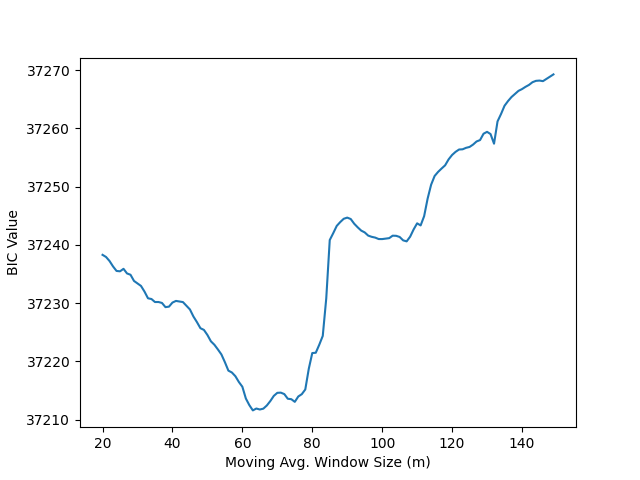
\includegraphics[width=\linewidth]{Prop_ST_Cr}
\end{subfigure}\hfill
\begin{subfigure}[!ht]{0.45\textwidth}
    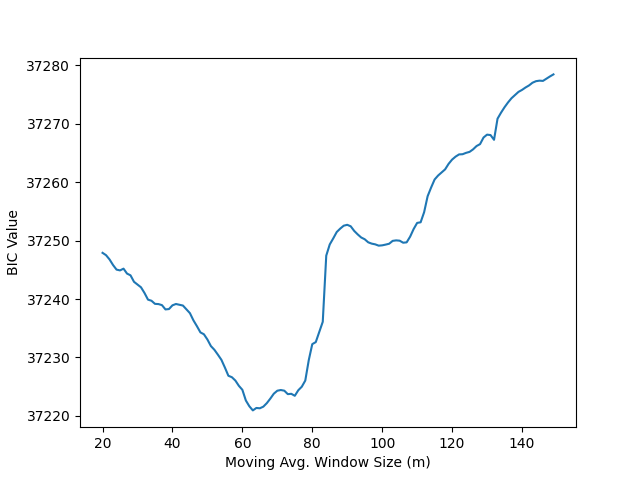
\includegraphics[width=\linewidth]{ST_Cr}
  \end{subfigure}

  \begin{subfigure}[!ht]{0.45\textwidth}
    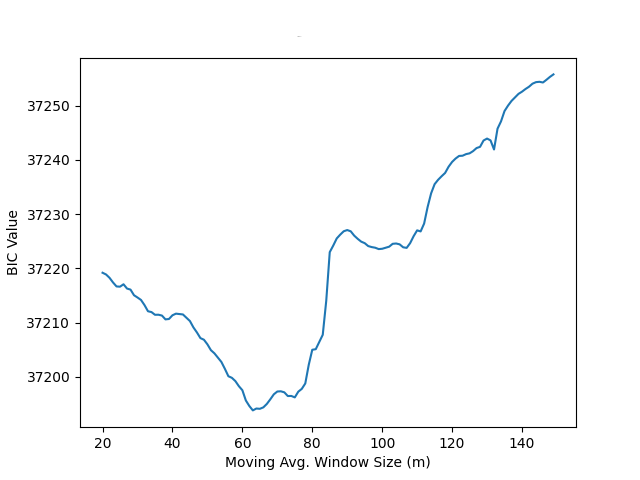
\includegraphics[width=\linewidth]{Prop_LT_Cr}
  \end{subfigure}\hfill
  \begin{subfigure}[!ht]{0.45\textwidth}
    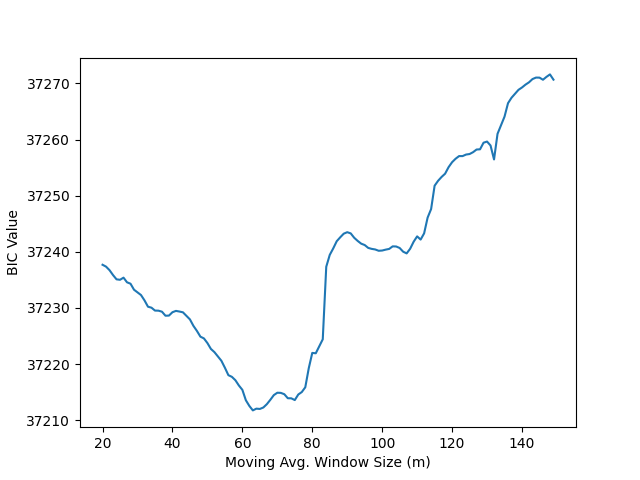
\includegraphics[width=\linewidth]{LT_Cr}
  \end{subfigure}

  \begin{subfigure}[!ht]{0.45\textwidth}
    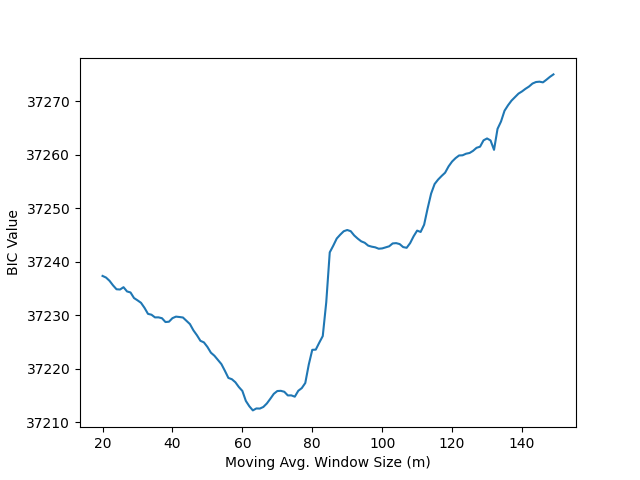
\includegraphics[width=\linewidth]{Prop_Both_Cr}
  \end{subfigure}\hfill
  \begin{subfigure}[!ht]{0.45\textwidth}
    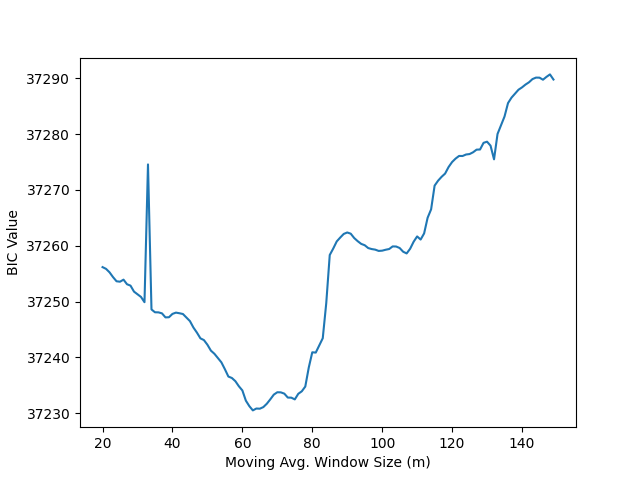
\includegraphics[width=\linewidth]{Both_Cr}
  \end{subfigure}

  \begin{subfigure}[!ht]{0.45\textwidth}
    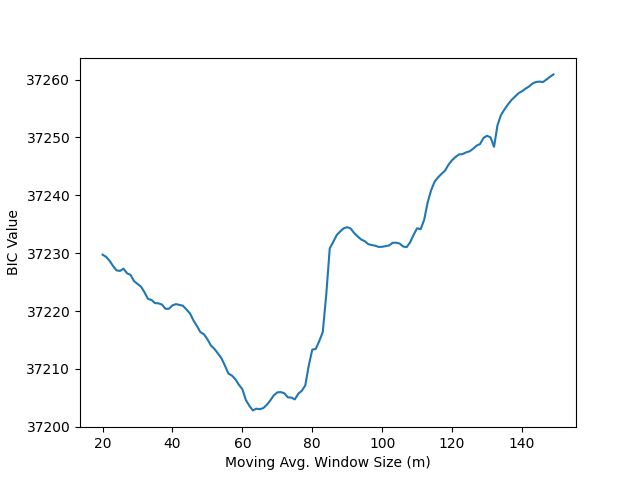
\includegraphics[width=\linewidth]{Prop_Vol_Cr}
  \end{subfigure}\hfill
  \begin{subfigure}[!ht]{0.45\textwidth}
    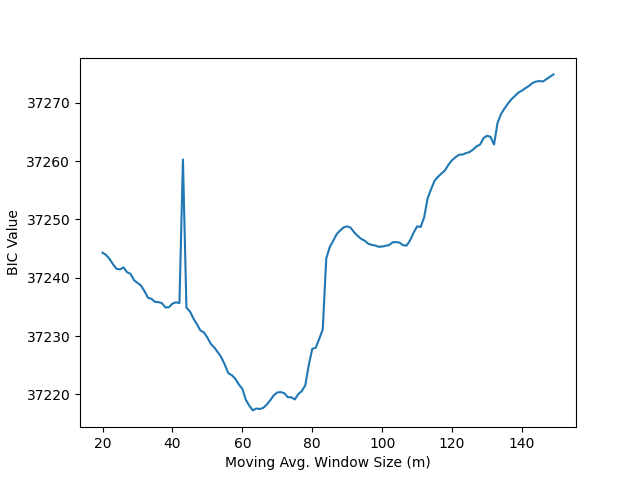
\includegraphics[width=\linewidth]{Vol_Cr}
  \end{subfigure}

\end{figure}

\pagebreak
%\restoregeometry
%\newgeometry{a4paper, margin=0.5in}
\section*{Tables}
\begin{table}[!ht]
\centering
\caption{Parameter Values for Monte Carlo Simulations}
\begin{tabular}{ccccccccccc}
\midrule
\midrule
$\alpha$ & $\gamma$ & $\beta$ & $\lambda_0$ & $\lambda_1$ & $\lambda_2$ & $\delta_0$ & $\delta_{1,s}$ & $\delta_{1,l}$ & $\delta_{1}$\\
\midrule
\multicolumn{11}{c}{\textbf{Short-term component}}\\
\multicolumn{11}{l}{\textbf{Proportional}}\\
0.006 & 0.160 & 0.842 & 0.011 & 0.085 & 0.902 & - & 0.027 & - & -\\
\multicolumn{11}{l}{\textbf{Non-Proportional}}\\
0.006 & 0.160 & 0.842 & 0.011 & 0.085 & 0.902 & 0.033 & -0.003 & - & -\\
\midrule
\multicolumn{11}{c}{\textbf{Long-term component}}\\
\multicolumn{11}{l}{\textbf{Proportional}}\\
0.006 & 0.160 & 0.842 & 0.011 & 0.085 & 0.902 & - & - & 0.049  & -\\
\multicolumn{11}{l}{\textbf{Non-Proportional}}\\
0.006 & 0.160 & 0.842 & 0.011 & 0.085 & 0.902 & 0.003 & - & 0.045 & -\\
\midrule
\multicolumn{11}{c}{\textbf{Both components (additive)}}\\
\multicolumn{11}{l}{\textbf{Proportional}}\\
0.006 & 0.160 & 0.842 & 0.011 & 0.085 & 0.902 & - & -0.005 & 0.054 & -\\
\multicolumn{11}{l}{\textbf{Non-Proportional}}\\
0.006 & 0.160 & 0.842 & 0.011 & 0.085 & 0.902 & 0.008 & -0.008 & 0.046 & -\\
\midrule
\multicolumn{11}{c}{\textbf{Overall conditional variance (multiplicative)}}\\
\multicolumn{11}{l}{\textbf{Proportional}}\\
0.006 & 0.160 & 0.842 & 0.011 & 0.085 & 0.902 & - & - & - & 0.042\\
\multicolumn{11}{l}{\textbf{Non-Proportional}}\\
0.006 & 0.160 & 0.842 & 0.011 & 0.085 & 0.902 & 0.020 & - & - & 0.023\\
\midrule
\multicolumn{11}{l}{\textbf{Notes:} This table presents the "true" parameter values I used in Monte Carlo}\\
\multicolumn{11}{l}{simulations of daily market premium data. The MF2-GARCH-in-mean model}\\
\multicolumn{11}{l}{is fitted $R=1,000$ times on these simulated samples, each of size $T=15,120$.}\\
\multicolumn{11}{l}{This is repeated for the proportional and non-proportional variant of every}\\
\multicolumn{11}{l}{specification. These values were chosen based on estimates from real data \textit{(see}}\\
\multicolumn{11}{l}{\textit{Table 4 below).}}\\
\midrule
\midrule
\end{tabular}
\end{table}

\begin{table}[!ht]
\centering
\caption{Summary Statistics - Market Premia}
\begin{tabular}{cccccccc}
\midrule
\midrule
\mbox{} & mean & sd & skew & kurtosis & min & max & AC(1)\\
\midrule
$r_t$ & 0.028 & 1.028 & -0.487 & 15.564 & -17.440 & 11.360 & 0.016\\
\midrule
\multicolumn{8}{l}{\textbf{Notes:} This table shows summary statistics for the U.S. daily}\\
\multicolumn{8}{l}{market premium data. The data runs from January 1964 to April}\\
\multicolumn{8}{l}{2025. The columns present the mean, standard deviation (sd),}\\
\multicolumn{8}{l}{skewness, kurtosis, minimum (min), maximum (max) and the}\\
\multicolumn{8}{l}{first-order autocorrelation coefficient (AC(1)).}\\
\midrule
\midrule
\end{tabular}
\end{table}

\begin{table}[!ht]
\centering
\caption{NBER Recession Periods}
\begin{tabular}{ccl}
\midrule
\midrule
Start date & End date & Remarks\\
\midrule
December 1969 & November 1970 & - \\
November 1973 & March 1975 & 1973 oil crisis and stagflation \\
January 1980 & July 1980 & Volcker recession I \\
July 1981 & November 1982 & Volcker recession II \\
July 1990 & March 1991 & - \\
March 2001 & November 2001 & Dot-com bubble \\
December 2007 & June 2009 & Global financial crisis \\
February 2020 & April 2020 & COVID-19 pandemic \\
\midrule
\multicolumn{3}{l}{\textbf{Notes:} This table shows the start and end dates of recession}\\
\multicolumn{3}{l}{periods defined by the U.S. National Bureau of Economic}\\
\multicolumn{3}{l}{Research (NBER) which fall within the sample period on which}\\
\multicolumn{3}{l}{the MF2-GARCH-in-mean model is estimated. The dummy}\\
\multicolumn{3}{l}{variable used to control for periods of crisis is given the value 1}\\
\multicolumn{3}{l}{for the above periods and 0 otherwise.}\\
\midrule
\midrule
\end{tabular}
\end{table}

\pagebreak
\restoregeometry
\newgeometry{a4paper, margin=0.5in}

\begin{sidewaystable}[!ht]
\centering
\scriptsize                           % smaller font
\setlength{\tabcolsep}{3pt}           % reduce horizontal padding
\renewcommand{\arraystretch}{0.8}     % reduce vertical padding
\caption{Combined Specification Parameter Estimates (Controlling for Crises)}
\resizebox{\textwidth}{!}{%
  \begin{tabular}{ccccccccccccccccc}
    \toprule\toprule
    $\alpha$ & $\gamma$ & $\beta$ & $\lambda_0$ & $\lambda_1$ & $\lambda_2$ & $\delta_0$ & $\delta_{1,s}$ & $\delta_{1,l}$ & $\delta_{1}$ & $\theta_0$ & $\theta_{1,s}$ & $\theta_{1,l}$ & $\theta_{1}$ & LLF & BIC \\
    \midrule
    \multicolumn{17}{c}{\textbf{Panel A: Short-term component}}\\
    \multicolumn{17}{l}{\textbf{Proportional}}\\
    \begin{tabular}[t]{@{}c@{}}0.007 \\ (0.014)\end{tabular} &
    \begin{tabular}[t]{@{}c@{}}0.158*** \\ (0.019)\end{tabular} &
    \begin{tabular}[t]{@{}c@{}}0.841*** \\ (0.018)\end{tabular} &
    \begin{tabular}[t]{@{}c@{}}0.012 \\ (0.020)\end{tabular} &
    \begin{tabular}[t]{@{}c@{}}0.086 \\ (0.150)\end{tabular} &
    \begin{tabular}[t]{@{}c@{}}0.900*** \\ (0.173)\end{tabular} &
    - &
    \begin{tabular}[t]{@{}c@{}}0.027** \\ (0.011)\end{tabular} &
    - & - & - &
    \begin{tabular}[t]{@{}c@{}}-0.013 \\ (0.020)\end{tabular} &
    - & - & -18567 & 37212 \\
    \multicolumn{17}{l}{\textbf{Non‑Proportional}}\\
    \begin{tabular}[t]{@{}c@{}}0.005* \\ (0.003)\end{tabular} &
    \begin{tabular}[t]{@{}c@{}}0.166*** \\ (0.015)\end{tabular} &
    \begin{tabular}[t]{@{}c@{}}0.845*** \\ (0.012)\end{tabular} &
    \begin{tabular}[t]{@{}c@{}}0.011*** \\ (0.002)\end{tabular} &
    \begin{tabular}[t]{@{}c@{}}0.081*** \\ (0.018)\end{tabular} &
    \begin{tabular}[t]{@{}c@{}}0.907*** \\ (0.018)\end{tabular} &
    \begin{tabular}[t]{@{}c@{}}0.033*** \\ (0.007)\end{tabular} &
    \begin{tabular}[t]{@{}c@{}}-0.003*** \\ (0.001)\end{tabular} &
    - & - &
    \begin{tabular}[t]{@{}c@{}}0.009 \\ (0.008)\end{tabular} &
    \begin{tabular}[t]{@{}c@{}}-0.009 \\ (0.009)\end{tabular} &
    - & - & -18562 & 37221 \\
    \multicolumn{17}{l}{LRT: 9.928***}\\
    \midrule

    \multicolumn{17}{c}{\textbf{Panel B: Long-term component}}\\
    \multicolumn{17}{l}{\textbf{Proportional}}\\
    \begin{tabular}[t]{@{}c@{}}0.006** \\ (0.003)\end{tabular} &
    \begin{tabular}[t]{@{}c@{}}0.160*** \\ (0.015)\end{tabular} &
    \begin{tabular}[t]{@{}c@{}}0.842*** \\ (0.013)\end{tabular} &
    \begin{tabular}[t]{@{}c@{}}0.011*** \\ (0.003)\end{tabular} &
    \begin{tabular}[t]{@{}c@{}}0.085*** \\ (0.018)\end{tabular} &
    \begin{tabular}[t]{@{}c@{}}0.902*** \\ (0.020)\end{tabular} &
    - & - &
    \begin{tabular}[t]{@{}c@{}}0.049*** \\ (0.009)\end{tabular} &
    - & - & - &
    \begin{tabular}[t]{@{}c@{}}-0.002*** \\ (0.001)\end{tabular} &
    - & -18558 & \textbf{37194} \\
    \multicolumn{17}{l}{\textbf{Non‑Proportional}}\\
    \begin{tabular}[t]{@{}c@{}}0.006* \\ (0.004)\end{tabular} &
    \begin{tabular}[t]{@{}c@{}}0.161*** \\ (0.015)\end{tabular} &
    \begin{tabular}[t]{@{}c@{}}0.843*** \\ (0.014)\end{tabular} &
    \begin{tabular}[t]{@{}c@{}}0.011* \\ (0.006)\end{tabular} &
    \begin{tabular}[t]{@{}c@{}}0.080*** \\ (0.030)\end{tabular} &
    \begin{tabular}[t]{@{}c@{}}0.907*** \\ (0.036)\end{tabular} &
    \begin{tabular}[t]{@{}c@{}}0.003 \\ (0.003)\end{tabular} &
    - &
    \begin{tabular}[t]{@{}c@{}}0.045*** \\ (0.017)\end{tabular} &
    - &
    \begin{tabular}[t]{@{}c@{}}-0.054 \\ (0.060)\end{tabular} &
    - &
    \begin{tabular}[t]{@{}c@{}}0.049 \\ (0.049)\end{tabular} &
    - & -18558 & 37212 \\
    \multicolumn{17}{l}{LRT: 1.358}\\
    \midrule

    \multicolumn{17}{c}{\textbf{Panel C: Both components (additive)}}\\
    \multicolumn{17}{l}{\textbf{Proportional}}\\
    \begin{tabular}[t]{@{}c@{}}0.006 \\ (0.013)\end{tabular} &
    \begin{tabular}[t]{@{}c@{}}0.161*** \\ (0.015)\end{tabular} &
    \begin{tabular}[t]{@{}c@{}}0.844*** \\ (0.016)\end{tabular} &
    \begin{tabular}[t]{@{}c@{}}0.012* \\ (0.006)\end{tabular} &
    \begin{tabular}[t]{@{}c@{}}0.085** \\ (0.035)\end{tabular} &
    \begin{tabular}[t]{@{}c@{}}0.901*** \\ (0.042)\end{tabular} &
    - &
    \begin{tabular}[t]{@{}c@{}}-0.005 \\ (0.021)\end{tabular} &
    \begin{tabular}[t]{@{}c@{}}0.054** \\ (0.023)\end{tabular} &
    - & - &
    \begin{tabular}[t]{@{}c@{}}-0.012** \\ (0.006)\end{tabular} &
    \begin{tabular}[t]{@{}c@{}}0.009 \\ (0.012)\end{tabular} &
    - & -18558 & 37212 \\
    \multicolumn{17}{l}{\textbf{Non‑Proportional}}\\
    \begin{tabular}[t]{@{}c@{}}0.006 \\ (0.003)\end{tabular} &
    \begin{tabular}[t]{@{}c@{}}0.162*** \\ (0.016)\end{tabular} &
    \begin{tabular}[t]{@{}c@{}}0.844*** \\ (0.014)\end{tabular} &
    \begin{tabular}[t]{@{}c@{}}0.011 \\ (0.007)\end{tabular} &
    \begin{tabular}[t]{@{}c@{}}0.081** \\ (0.036)\end{tabular} &
    \begin{tabular}[t]{@{}c@{}}0.906*** \\ (0.043)\end{tabular} &
    \begin{tabular}[t]{@{}c@{}}0.008 \\ (0.006)\end{tabular} &
    \begin{tabular}[t]{@{}c@{}}-0.008 \\ (0.007)\end{tabular} &
    \begin{tabular}[t]{@{}c@{}}0.046*** \\ (0.012)\end{tabular} &
    - &
    \begin{tabular}[t]{@{}c@{}}-0.050 \\ (0.067)\end{tabular} &
    \begin{tabular}[t]{@{}c@{}}-0.002 \\ (0.002)\end{tabular} &
    \begin{tabular}[t]{@{}c@{}}0.048 \\ (0.041)\end{tabular} &
    - & -18557 & 37230 \\
    \multicolumn{17}{l}{LRT: 0.990}\\
    \midrule

    \multicolumn{17}{c}{\textbf{Panel D: Overall conditional variance (multiplicative)}}\\
    \multicolumn{17}{l}{\textbf{Proportional}}\\
    \begin{tabular}[t]{@{}c@{}}0.007 \\ (0.009)\end{tabular} &
    \begin{tabular}[t]{@{}c@{}}0.158*** \\ (0.016)\end{tabular} &
    \begin{tabular}[t]{@{}c@{}}0.839*** \\ (0.014)\end{tabular} &
    \begin{tabular}[t]{@{}c@{}}0.011** \\ (0.005)\end{tabular} &
    \begin{tabular}[t]{@{}c@{}}0.080*** \\ (0.031)\end{tabular} &
    \begin{tabular}[t]{@{}c@{}}0.907*** \\ (0.035)\end{tabular} &
    - & - & - &
    \begin{tabular}[t]{@{}c@{}}0.042*** \\ (0.010)\end{tabular} &
    - & - & - &
    \begin{tabular}[t]{@{}c@{}}-0.014* \\ (0.008)\end{tabular} &
    -18563 & 37203 \\
    \multicolumn{17}{l}{\textbf{Non‑Proportional}}\\
    \begin{tabular}[t]{@{}c@{}}0.006 \\ (0.012)\end{tabular} &
    \begin{tabular}[t]{@{}c@{}}0.162*** \\ (0.025)\end{tabular} &
    \begin{tabular}[t]{@{}c@{}}0.841*** \\ (0.018)\end{tabular} &
    \begin{tabular}[t]{@{}c@{}}0.011 \\ (0.016)\end{tabular} &
    \begin{tabular}[t]{@{}c@{}}0.080 \\ (0.084)\end{tabular} &
    \begin{tabular}[t]{@{}c@{}}0.908*** \\ (0.101)\end{tabular} &
    \begin{tabular}[t]{@{}c@{}}0.020 \\ (0.059)\end{tabular} &
    - & - &
    \begin{tabular}[t]{@{}c@{}}0.023 \\ (0.083)\end{tabular} &
    \begin{tabular}[t]{@{}c@{}}-0.005 \\ (0.016)\end{tabular} &
    - & - &
    \begin{tabular}[t]{@{}c@{}}-0.004 \\ (0.022)\end{tabular} &
    -18560 & 37217 \\
    \multicolumn{17}{l}{LRT: 4.850*}\\
    \midrule
\multicolumn{17}{l}{\textbf{Notes:} This table shows the results of the QMLE parameter estimates for the MF2-GARCH-in-mean model. The numbers in parentheses are Bollerslev-}\\
\multicolumn{17}{l}{Wooldridge robust standard errors. *** ,** and * indicate significance at the 1\%, 5\% and 10\% level. Each panel shows the results for a different}\\
\multicolumn{17}{l}{specification, depending on which components of volatility are included. Each panel shows the proportional (no intercept) and non-proportional}\\
\multicolumn{17}{l}{variant. The likelihood ratio test (LRT) statistic for the proportional variant against the non-proportional variant is also shown at the bottom of each}\\
\multicolumn{17}{l}{panel. All specifications are estimated using daily U.S. market premium data for the period January 1964 to April 2025 inclusive. The moving average}\\
\multicolumn{17}{l}{window size (m) which minmizes the Bayesian Information Criterion for all specifications is m=63.}\\
\midrule
\midrule
  \end{tabular}%
}
\end{sidewaystable}


\pagebreak
\restoregeometry
%\newgeometry{a4paper, margin=0.2in}
\begin{table}[!ht]
\centering
\caption{Summary Statistics - Volatility}
\begin{tabular}{ccccc}
\multicolumn{5}{c}{(Proportional Long-Term Component Specification)}\\
\midrule
\midrule
\mbox{} & mean & min & max & AC(1)\\
\midrule
\mbox{$\sigma^2_t$}& 1.051 & 0.122 & 60.992 & 0.94736\\
\mbox{$h_t$} & 1.186 & 0.474 & 69.731 & 0.98251\\
\mbox{$\tau_t$} & 0.830 & 0.236 & 3.810 & 0.99988\\
\midrule
\multicolumn{5}{l}{\textbf{Notes:} This table shows summary statistics for}\\
\multicolumn{5}{l}{the conditional variance and its components as}\\
\multicolumn{5}{l}{estimated by MF2-GARCH in the proportional}\\
\multicolumn{5}{l}{(no intercept) long-term component specification.}\\
\midrule
\midrule
\end{tabular}
\end{table}

\pagebreak
\newgeometry{a4paper, margin=0.5in}
\begin{table}[!ht]
  \centering
  \scriptsize
  \setlength\tabcolsep{3pt}
  \caption{Monte Carlo Parameter Estimates \& Standard Deviations}
  % auto-scale to full text width
  \resizebox{\linewidth}{!}{%
    \begin{tabular}{lccccccccccc}
      \toprule
      & $\alpha$ & $\gamma$ & $\beta$ & $\lambda_0$ & $\lambda_1$ & $\lambda_2$ 
      & $\delta_0$ & $\delta_{1,s}$ & $\delta_{1,l}$ & $\delta_{1}$\\
      \midrule
      \multicolumn{12}{c}{\textbf{Short-term component}}\\
      \multicolumn{12}{l}{\textbf{Proportional}}\\
      True & 0.00600 & 0.16000 & 0.84200 & 0.01100 & 0.08500 & 0.90200 & - & 0.02700 & - & -\\
      Bias & -0.00116 & -0.00128 & 0.00198 & 0.00082 & 0.00119 & -0.00226 & - & -0.00011 & - & -\\
      (\%)  & (-19.33\%) & (-0.80\%) & (0.24\%) & (7.45\%) & (1.40\%) & (-0.25\%) & - & (-0.41\%) & - & -\\
      S.d.  & 0.00353 & 0.00684 & 0.00675 & 0.00601 & 0.03777 & 0.04460 & - & 0.00468 & - & -\\
      \addlinespace
      \multicolumn{12}{l}{\textbf{Non-Proportional}}\\
      True & 0.00600 & 0.16000 & 0.84200 & 0.01100 & 0.08500 & 0.90200 & 0.03300 & -0.00300 & - & -\\
      Bias & -0.00115 & -0.00072 & 0.00122 & 0.00086 & 0.00147 & -0.00259 & -0.00155 & 0.00150 & - & -\\
      (\%)  & (-19.17\%) & (-0.45\%) & (0.14\%) & (7.82\%) & (1.73\%) & (-0.29\%) & (-4.70\%) & (-50.00\%) & - & -\\
      S.d.  & 0.00356 & 0.00691 & 0.00711 & 0.00603 & 0.03789 & 0.04476 & 0.01192 & 0.01303 & - & -\\
      \midrule
      \multicolumn{12}{c}{\textbf{Long-term component}}\\
      \multicolumn{12}{l}{\textbf{Proportional}}\\
      True & 0.00600 & 0.16000 & 0.84200 & 0.01100 & 0.08500 & 0.90200 & - & - & 0.04900 & -\\
      Bias & -0.00116 & -0.00070 & 0.00139 & 0.00071 & 0.00052 & -0.00145 & - & - & -0.00010 & -\\
      (\%)  & (-19.33\%) & (-0.44\%) & (0.17\%) & (6.45\%) & (0.61\%) & (-0.16\%) & - & - & (-0.20\%) & -\\
      S.d.  & 0.00353 & 0.00693 & 0.00678 & 0.00578 & 0.03593 & 0.04253 & - & - & 0.00636 & -\\
      \addlinespace
      \multicolumn{12}{l}{\textbf{Non-Proportional}}\\
      True & 0.00600 & 0.16000 & 0.84200 & 0.01100 & 0.08500 & 0.90200 & 0.00300 & - & 0.04500 & -\\
      Bias & -0.00116 & -0.00070 & 0.00140 & 0.00073 & 0.00075 & -0.00170 & -0.00035 & - & 0.00022 & -\\
      (\%)  & (-19.33\%) & (-0.44\%) & (0.17\%) & (6.64\%) & (0.88\%) & (-0.19\%) & (-11.67\%) & - & (0.49\%) & -\\
      S.d.  & 0.00355 & 0.00692 & 0.00679 & 0.00577 & 0.03660 & 0.04314 & 0.01413 & - & 0.01833 & -\\
      \midrule
      \multicolumn{12}{c}{\textbf{Both components (additive)}}\\
      \multicolumn{12}{l}{\textbf{Proportional}}\\
      True & 0.00600 & 0.16000 & 0.84200 & 0.01100 & 0.08500 & 0.90200 & - & -0.00500 & 0.05400 & -\\
      Bias & -0.00116 & -0.00064 & 0.00124 & 0.00066 & 0.00050 & -0.00138 & - & 0.00057 & -0.00079 & -\\
      (\%)  & (-19.33\%) & (-0.40\%) & (0.15\%) & (6.00\%) & (0.59\%) & (-0.15\%) & - & (-11.40\%) & (-1.46\%) & -\\
      S.d.  & 0.00354 & 0.00692 & 0.00702 & 0.00563 & 0.03599 & 0.04239 & - & 0.01071 & 0.01272 & -\\
      \addlinespace
      \multicolumn{12}{l}{\textbf{Non-Proportional}}\\
      True & 0.00600 & 0.16000 & 0.84200 & 0.01100 & 0.08500 & 0.90200 & 0.00800 & -0.00800 & 0.04600 & -\\
      Bias & -0.00115 & -0.00061 & 0.00108 & 0.00068 & 0.00054 & -0.00145 & -0.00166 & 0.00156 & 0.00010 & -\\
      (\%)  & (-19.17\%) & (-0.38\%) & (0.13\%) & (6.18\%) & (0.64\%) & (-0.16\%) & (-20.75\%) & (-19.50\%) & (0.22\%) & -\\
      S.d.  & 0.00356 & 0.00693 & 0.00710 & 0.00568 & 0.03638 & 0.04281 & 0.01735 & 0.01309 & 0.01863 & -\\
      \midrule
      \multicolumn{12}{c}{\textbf{Overall conditional variance (multiplicative)}}\\
      \multicolumn{12}{l}{\textbf{Proportional}}\\
      True & 0.00600 & 0.16000 & 0.84200 & 0.01100 & 0.08500 & 0.90200 & - & - & - & 0.04200\\
      Bias & -0.00119 & -0.00144 & 0.00211 & 0.00077 & 0.00095 & -0.00195 & - & - & - & -0.00006\\
      (\%)  & (-19.83\%) & (-0.90\%) & (0.25\%) & (7.00\%) & (1.12\%) & (-0.22\%) & - & - & - & (-0.14\%)\\
      S.d.  & 0.00350 & 0.00682 & 0.00672 & 0.00594 & 0.03701 & 0.04378 & - & - & - & 0.00610\\
      \addlinespace
      \multicolumn{12}{l}{\textbf{Non-Proportional}}\\
      True & 0.00600 & 0.16000 & 0.84200 & 0.01100 & 0.08500 & 0.90200 & 0.02000 & - & - & 0.02300\\
      Bias & -0.00117 & -0.00109 & 0.00176 & 0.00081 & 0.00116 & -0.00221 & -0.00018 & - & - & 0.00011\\
      (\%)  & (-19.50\%) & (-0.68\%) & (0.21\%) & (7.36\%) & (1.36\%) & (-0.25\%) & (-0.90\%) & - & - & (0.48\%)\\
      S.d.  & 0.00353 & 0.00686 & 0.00689 & 0.00600 & 0.03745 & 0.04429 & 0.00846 & - & - & 0.01140\\
      \midrule
      \multicolumn{12}{l}{\textbf{Notes:} This table presents the results of MF2-GARCH-in-mean QMLE parameter estimation on data}\\
      \multicolumn{12}{l}{generated by Monte Carlo simulations of daily market premia. Each specification was fitted on a simulated}\\
      \multicolumn{12}{l}{sample of size $T=30,240$ and this was repeated $R=1,000$ times. The table shows the true parameter}\\
      \multicolumn{12}{l}{values (True), the average bias of the parameter estimates (value and percent), and the standard}\\
      \multicolumn{12}{l}{deviation (S.d.) of the parameter estimates across the 1,000 simulations.}\\
      \bottomrule
    \end{tabular}%
  }
\end{table}
\end{document}